\subsection{Eingabeknoten}

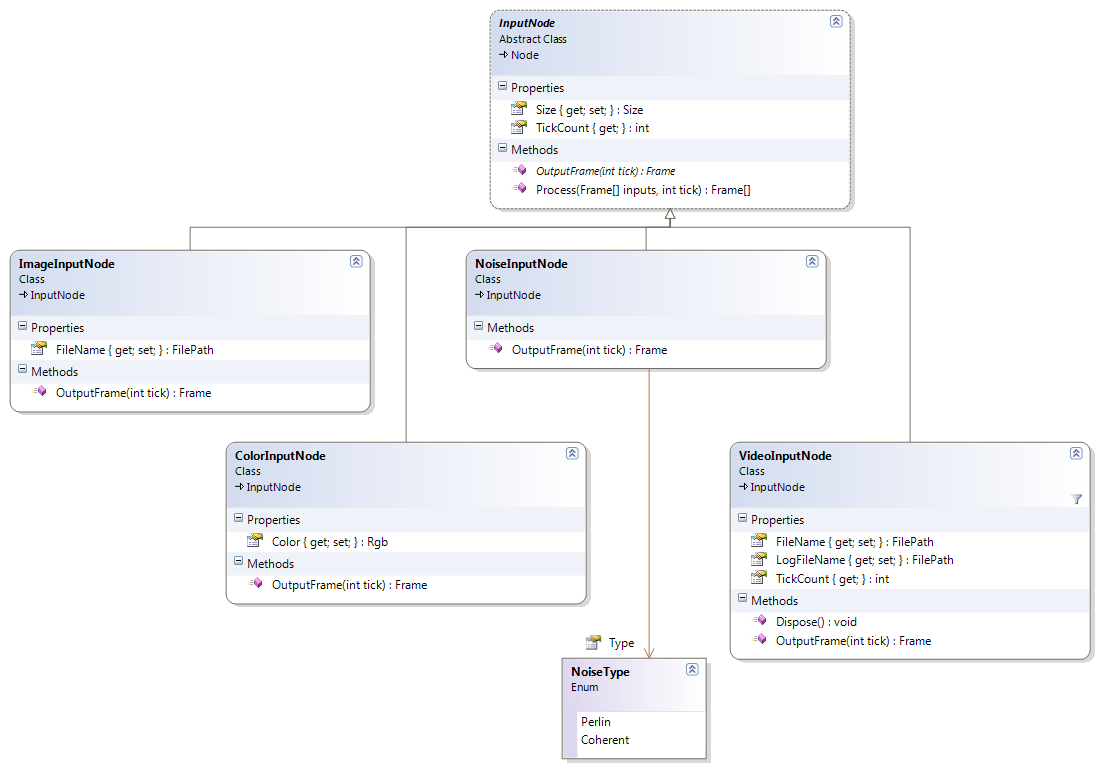
\includegraphics[width=\textwidth]{YuvKA.Pipeline/inputnodes.png}
Herpaderp Eingabeknoten derpa UML *Schnurrbartzwirbel*.

\subsubsection{YuvKA.Pipeline.InputNode}

\begin{verbatim}
[DataContract]
public abstract class InputNode : Node
\end{verbatim}

\paragraph{Beschreibung}~\\
Die abstrakte Klasse \name{InputNode} modelliert die Eingabequellen der Pipeline, und liefert eine gemeinsame Basis für deren konkrete Implementationen.

\paragraph{Typmember}
\begin{itemize}

\property{Size}
	\begin{verbatim}
	[DataMember]
	public Size Size{ get; set; }
	\end{verbatim}
	Spezifiziert die Größe des vom Knoten gelieferten \name{Frame}s in Form eines \name{Size}-Objektes.

\property{FrameCount}
	\begin{verbatim}
	[DataMember]
	public virtual int FrameCount { get; }
	\end{verbatim}
	Ruft die Anzahl an vom Knoten zu liefernden \name{Frame}s ab. Der Standardrückgabewert ist 1, die Methode ist allerdings in Unterklassen überschreibbar.

\end{itemize}

\subsubsection{YuvKA.Pipeline.ColorInputNode}

\subsubsection{YuvKA.Pipeline.NoiseInputNode}

\subsubsection{YuvKA.Pipeline.ImageInputNode}

\subsubsection{YuvKA.Pipeline.VideoInputNode}
